% No modificar estas líneas de código, por favor dirigirse a ANEXOS más abajo.

            \newpage
            \addtocontents{toc}{\cftpagenumbersoff{section}} 
            \phantomsection\addcontentsline{toc}{section}{ANEXOS}
            \addtocontents{toc}{\cftpagenumberson{section}}
            
            \newcommand{\anex}[1]
            {
                \newpage
                \vspace*{\fill}
                \section{#1}
                \label{anx:#1}
                \vspace*{\fill}
                \newpage
            }
            
            \appendix
            \renewcommand{\thesection}{\arabic{section}}
            \addtocontents{toc}
            {
                \protect\renewcommand{\protect\cftsecfont}{\normalfont}%
                \protect\renewcommand{\protect\cftsecpresnum}{Anexo }
                \setlength{\cftsecnumwidth}{1.8cm}
                \setlength{\cftbeforesecskip}{-8pt}%
            }
            %\addtocontents{toc}{\setlength{\cftbeforesecskip}{-4pt}}
            %\addtocontents{toc}{\setlength{\cftsecnumwidth}{1.8cm}}
            %\addtocontents{toc}{\protect\setstretch{1.2}}
            %\addtocontents{toc}{\cftsecpagefont}{}
            
            \setcounter{page}{1}
            \setcounter{figure}{0}
            \setcounter{table}{0}
            \titleformat{\section}{\bfseries\normalsize\flushright}{\MakeUppercase{\textbf{ANEXO }\thesection}}{0em}{\\ \MakeUppercase}
            \captionsetup{list=no} % Para que no aparezca en índice general 

            
%Los comandos \verb|\anex{}| y \verb|\apex{}| crean una hoja de anexo o apéndice con el título que se le asigne. 

%Para referenciar anexos o apéndices existen los comandos \verb|\anx{}| y \verb|\apx{}| que funcionan con el mismo título del anexo o apéndice.
%------------------------
%
%       ANEXOS
%
%------------------------

\anex{Datasheet de ESP32 C3}
\label{anx:1}
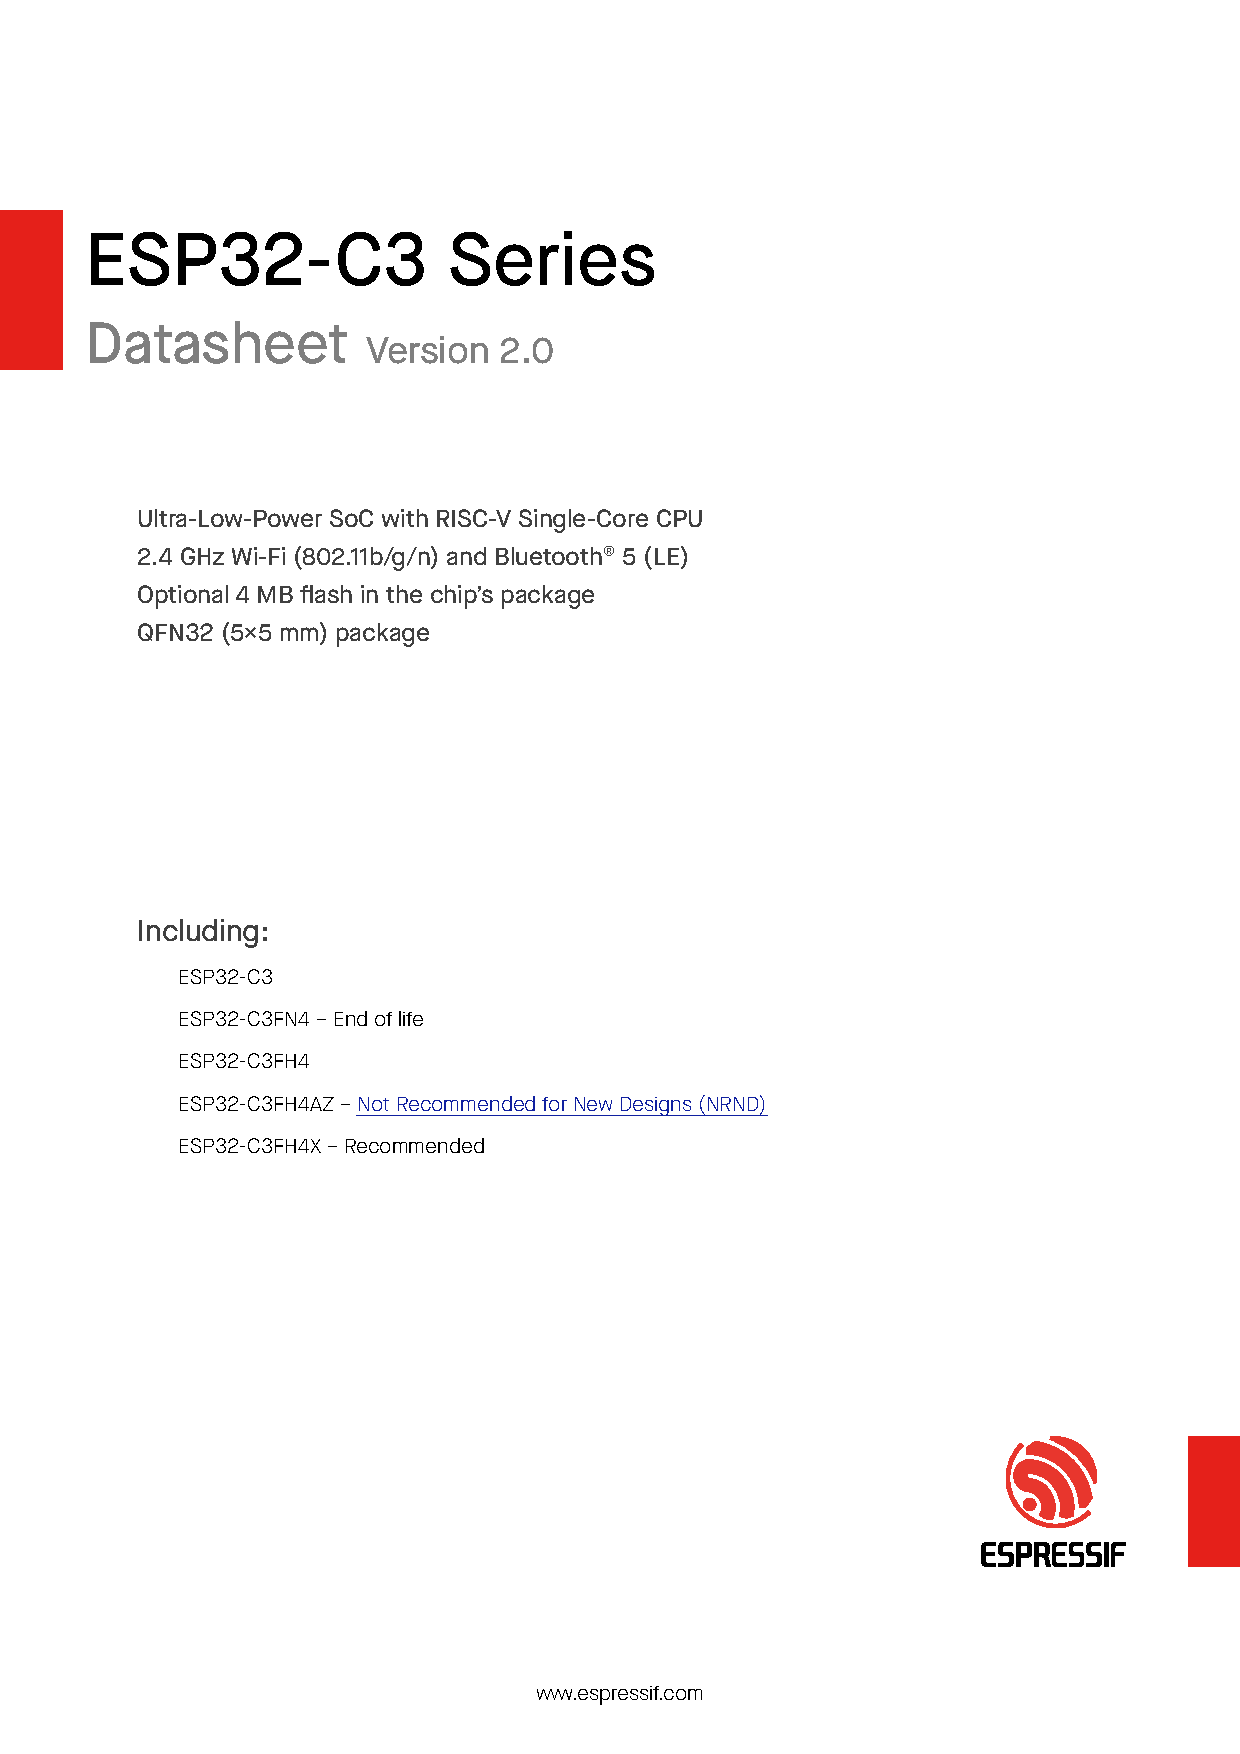
\includepdf[pages={1,2,3,4,5}]{PDFs/esp32-c3_datasheet.pdf}

\anex{Datasheet de MAX485}
\label{anx:2}
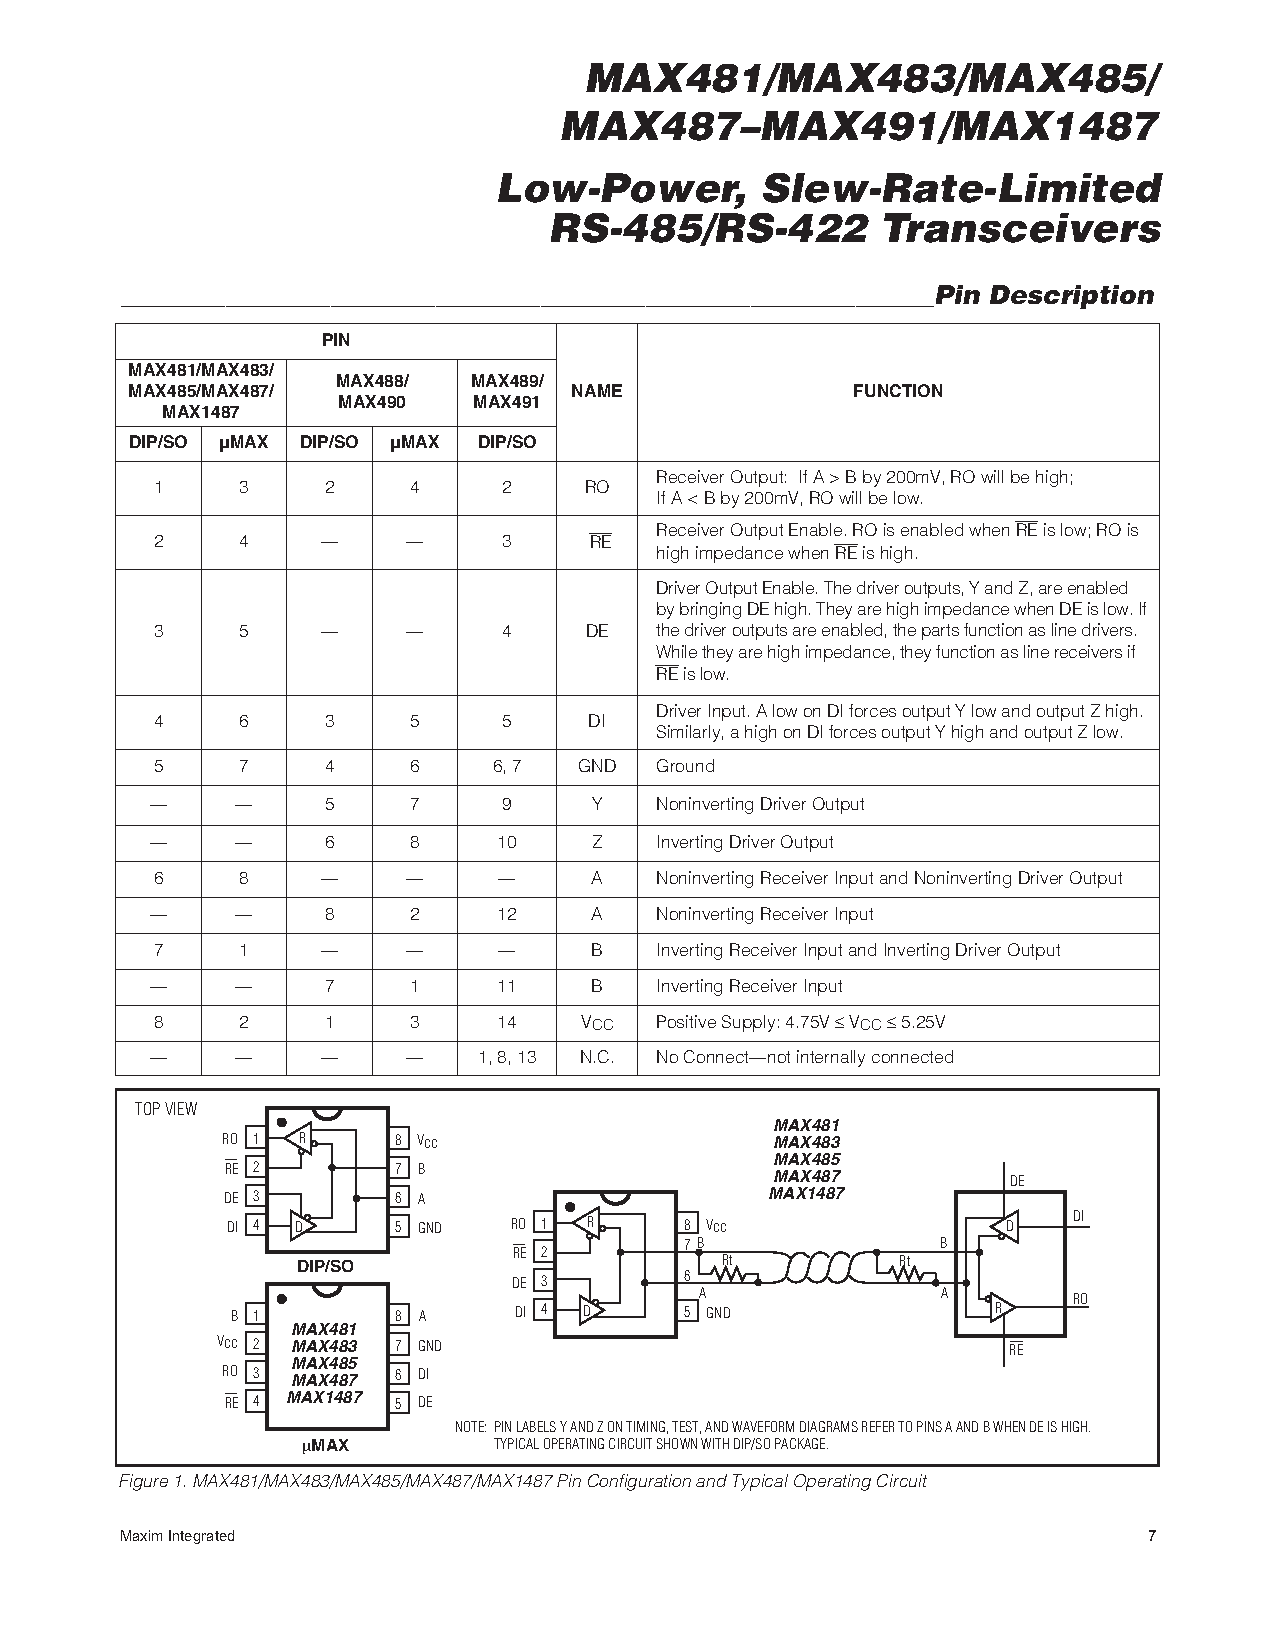
\includepdf[pages={1,2}]{PDFs/max485.pdf}
